\documentclass[9pt, compress, xcolor=table]{beamer}


\usetheme{m}

\usepackage{amsmath,amssymb,amsthm}
\usepackage{latexsym}
\usepackage{booktabs}
\usepackage[scale=2]{ccicons}
\usepackage{minted}
\usepackage[english, russian]{babel}
\usepackage{graphicx}
\usepackage{xcolor}
\usepackage{euscript}
% \DeclareMathOperator{\arctg}{arctg}
\usepackage{tabu} % https://ru.sharelatex.com/learn/Tables
\DeclareGraphicsExtensions{.pdf,.jpg,.png}
\graphicspath{{../images/}{./images/}}

\colorlet{Mycolor1}{green!50!blue!50!}
\DeclareMathOperator{\Ima}{Im}
\usemintedstyle{trac}

\title{Физические принципы оптической микроскопии сверхвысокого разрешения}
\subtitle{осенний семестр, 2015}
\author{ассистент, к.ф.-м.н. Шутова О.А.}
\institute{МГУ им. М.В. Ломоносова, физический факультет}

\begin{document}

\maketitle

\plain{}{Лекция 10. Активные плазмонные материалы}

\begin{frame}{Идея лекции}

На позапрошлой лекции мы говорили о том, что основной проблемой для метаматериалов в оптическом диапазоне являются большие потери. При создании композита мы вынуждены использовать как металл, так и диэлектрик. 

Одним из вариантов уменьшения потерь является поиск диэлектрика с наименьшими потерями, такого как оксид титана.

На прошлой лекции мы рассматривали такие конфигурации эксперимента, когда наноструктурированный металл разделен слоями воздуха.

Однако все эти варианты не дают желаемого результата по качеству разрешения и количеству потерь.

Еще одним принципиально иным спобом является создание т.н. активного плазмонного материала. В этом случае диэлектрик может быть заменен на активную среду. Роль активной среды может играть слой флуоресцентных молекул или полупроводниковые точки/колодцы.

\end{frame}

\begin{frame}{Нанолазер}

Нанолазер - это объект, возникающий при помещении активной среды внутрь наноструктурированного металла, это может быть дипольный нанолазер, спазер, лазер на магнитной моде.

Активная среда, как и в случае лазера, может быть промоделирована 4-мя уровнями, однако, в отличие от активной среды лазера безызлучательно передает энергию на рабочем уровне. При этом на границе наноструктурированного материала возбуждаются и усиливаются поверхностные плазмоны, играющие роль фотонов в резонаторе.

Необходимо понимать важнейшие отличия спазеров от лазеров. Результатом работы лазера является коллимированный пучок когерентного света. В результате работы спазера мы не имеем пучка света. Это лишь поле поверхностных плазмонов, которое без дополнительных устройств мы не можем увидеть в дальней зоне.


\end{frame}

\begin{frame}{Литература}

\begin{itemize}
\item M. Noginov Demonstration of a spaser-based nanolaser. Nature, 2009 (первое экспериментальное подтверждение)
\item O. Hess, J. Pendry et al. Active nanoplasmonic metamaterials. Nature Materials. 2012. (обзор)
\item А.П. Виноградов и др. Квантовая плазмоника метаматериалов: перспективы компенсации потерь при помощи спазеров. УФН, 2012 (теория)
\item V. Shalaev et al. Loss-free and active optical negative-index metamaterials. Nature. 2010 (эксперимент, флуоресценция)
\end{itemize}



\end{frame}

\begin{frame}{Спазер на флуоресцентных молкулах}
\begin{center}
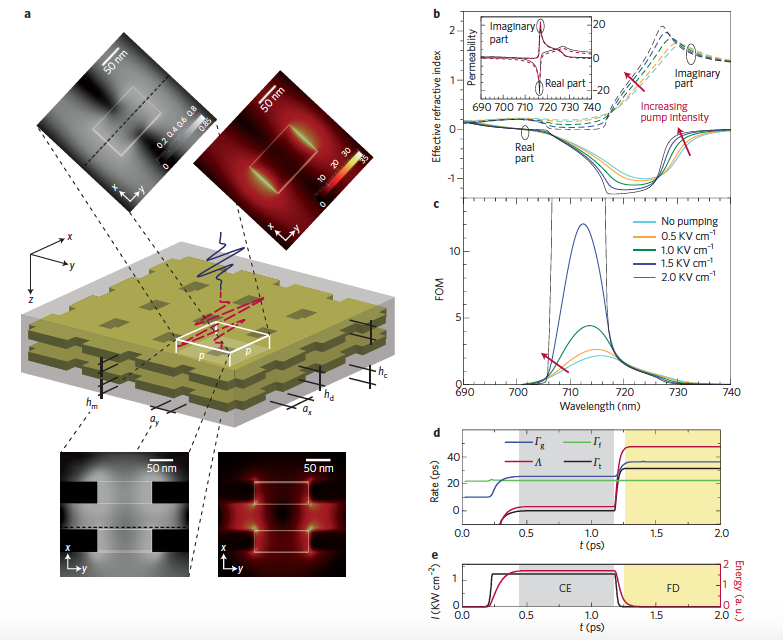
\includegraphics[width=0.65\textwidth]{am1}
\end{center}

{\small (a) Инверсия населенностей (слева) и электрическое поле (справа)

(b) Действительная и мнимая части показателя преломления в зависимости от напряженности накачки (от 0 кВ/см до 2кВ/см)

(с) $FOM=Re[n]/Im[n]$

(d) динамика диссипации и излучения энергии, CE - continious excitation, FD - free decay}
\end{frame}

\begin{frame}{}
\begin{center}
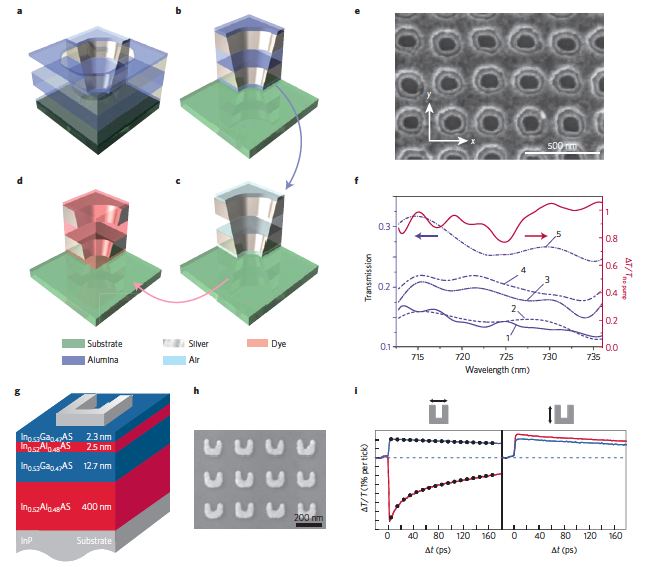
\includegraphics[width=0.8\textwidth]{am2}
\end{center}
Необходимо оптимизировать не только напряженность накачки, но и время задержки 

\end{frame}

\begin{frame}{}
\begin{center}
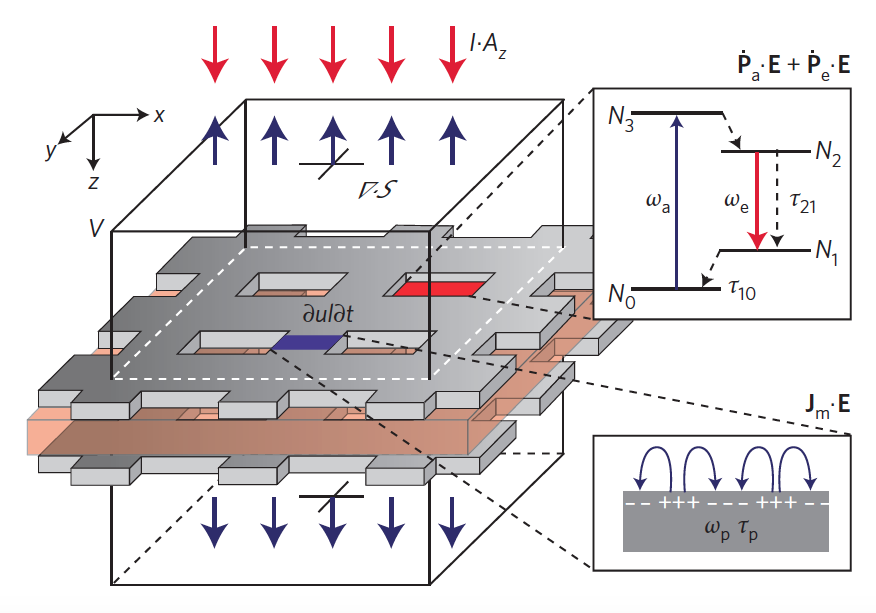
\includegraphics[width=0.9\textwidth]{am3}
\end{center}
\end{frame}

\begin{frame}{}
\begin{center}
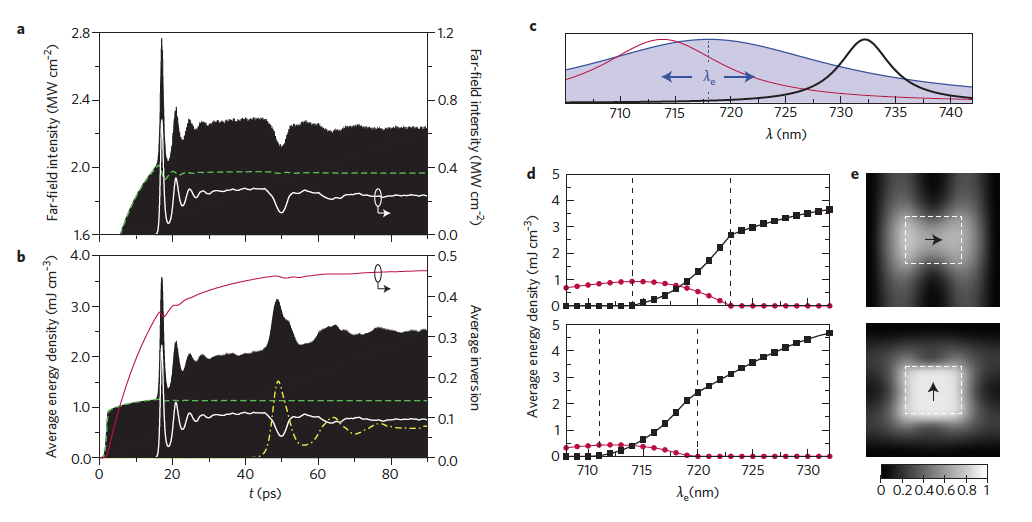
\includegraphics[width=0.9\textwidth]{am4}
\end{center}
\end{frame}

\begin{frame}{}
\begin{center}
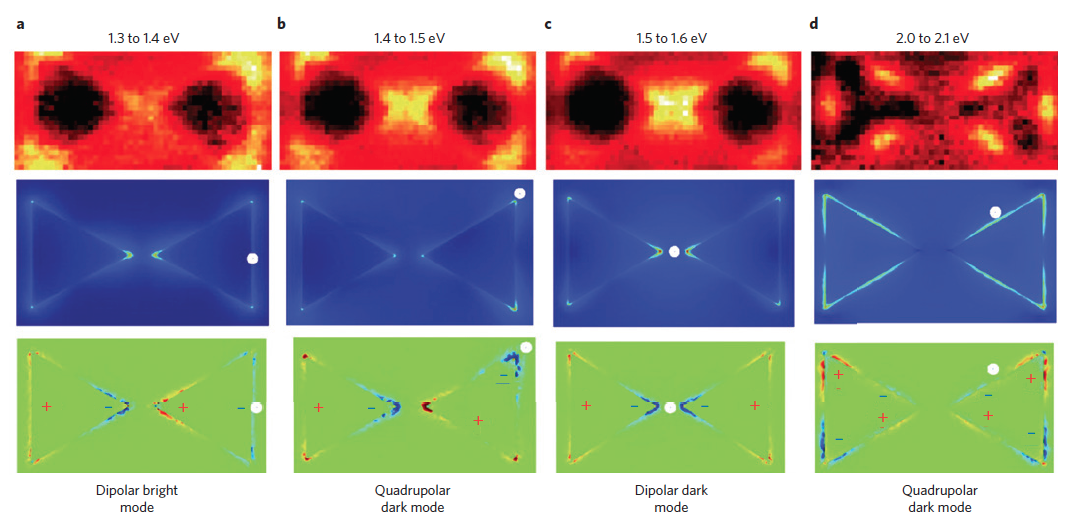
\includegraphics[width=0.9\textwidth]{am5}
\end{center}
\end{frame}

\begin{frame}{}
\begin{center}
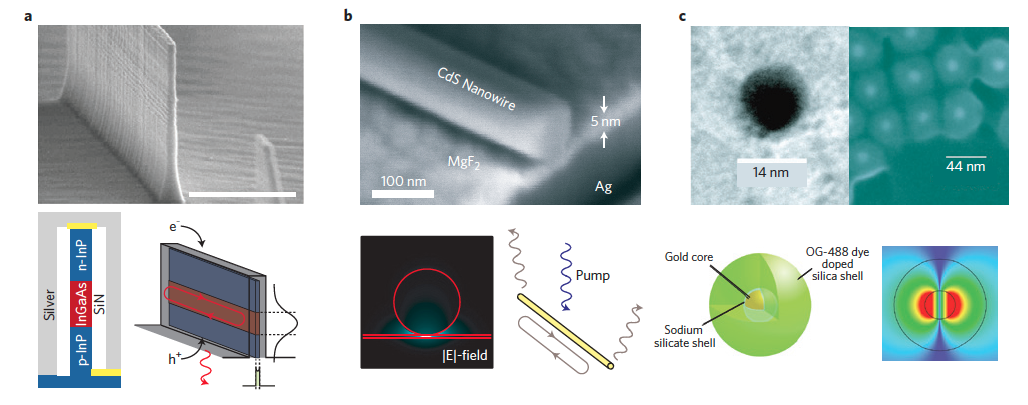
\includegraphics[width=0.9\textwidth]{am6}
\end{center}
\end{frame}

\begin{frame}{}
\begin{center}
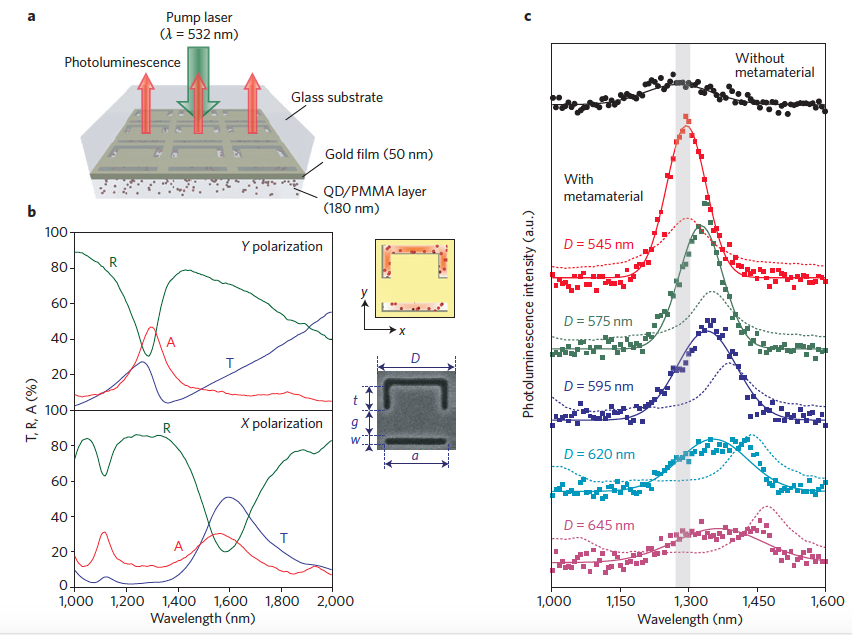
\includegraphics[width=0.9\textwidth]{am7}
\end{center}
\end{frame}


\end{document}


\begin{frame}{}
\begin{columns}[c]
\column{6.5cm}
\begin{center}
\includegraphics[width=0.9\textwidth]{}
\end{center}
\column{6.5cm}
\begin{center}
\includegraphics[width=0.9\textwidth]{}
\end{center}
\end{columns}
\end{frame}

\begin{frame}{}
\begin{center}
\includegraphics[width=0.9\textwidth]{}
\end{center}
\end{frame}